\section{Métriques de procédés}
\label{sec:metriques}

Nous décrivons dans cette partie comment les métriques de procédés sont calculés. Puis, nous expliquons comment les fichiers renommés peuvent avoir un impact sur ces métriques. Enfin, nous décrivons comment les VCS, actuellement, traitent le renommage.\\

\subsection{Calcul des métriques de procédés}

Les métriques de procédés (change metrics) permettent de calculer à quel point une entité de code source a été modifiée au cours d'une période donnée dans l'histoire d'un logiciel. Pour la prédiction de bugs, elles sont utilisés usuellement dans la dernière période, c'est à dire entre l'avant dernière et la dernière version du projet. L'objectif est de prédire les bugs qui apparaîtront lors de la prochaine version, en particulié si cette version est une \texttt{release}, c'est à dire une sortie de logiciel dite stable. Elles ne considèrent donc que les entités étant toujours présentes à la fin de la période et qui ont étés actives dans la période.\\

Un gestionnaire de versions (VCS) offre plusieurs moyens de calculer les métriques de procédés car il stocke les informations sur les entités modifiées à chaque nouvelle version, l'auteur de ces modifications, la date, etc. De plus, il permet la récupération du contenu de chaque entité et de l'ensemble d'un projet à une version donnée. Pour calculer ces métriques, il est donc possible d'analyser chaque entité modifiée lors d'une période puis de garder uniquement les entités toujours présentes à la dernière version de notre période.\\

Plus précisement, voici comment un VCS peut être utilisé pour calculer les trois métriques de procédés les plus utilisés: le nombre de développeurs (Number of Developers, NoD), le nombre de modifications  (Number of Changes, NoC) et le Code Churn (CC). 

\begin{enumerate}
\item  Nous récupérons d'abord la dernière version du projet pour obtenir les entités existantes à la fin de la période considérée. On note $A$ cet ensemble d'entités.
\item Toujours grâce aux commandes git, nous récupérons toutes les modifications effectuées durant la période. On note $C$ l'ensemble des modifications dans l'ordre chronologique.
\item  Troisièmement, nous parcourons cet ensemble de modifications en commençant par la plus ancienne ($c_0 \in C$) jusqu'à la plus récente ($c_n \in C$) dans le but de calculer les métriques de procédés pour chaque entité.
\end{enumerate}

 On note $\mu_{a}^{M}$ la valeur de la métrique $M$ pour l'entité $a$. Ensuite nous calculons les métriques comme suivant (on note $c_i$ la modification courante lors du parcours):

\begin{description}
	\item[NoD] (nombre de développeurs) Pour chaque entité $a$ pointé par $c_i$ qui appartient aussi à $A$ ($a \in A$), on ajoute à $\mu_{a}^{NoD}$ le nombre d'auteurs qui ont effectué les modifications $c_i$ et qui ont modifiés $a$ pour la première fois dans la période.
	\item[NoC] (nombre de modifications) Pour chaque entité $a$ pointé par $c_i$ qui appartient aussi à $A$ ($a \in A$), on ajoute $1$ à $\mu_{a}^{C}$ tels que $c_i$ indique qu'une nouvelle modification a été effectuée.
	\item[CC] (Code Churn) Pour chaque entité $a$ pointé par $c_i$ qui appartient aussi à $A$ ($a \in A$), on vérifie d'abord que la modification n'est pas une creation d'entité. Si c'est le cas celà veut dire que l'entité a été créée durant la période, donc on initialise son $\mu_{a}^{CC}$ à son nombre de lignes. Ensuite au prochain $c_j$ qui cible $a$ dans la période avec ($i < j$), on compare les deux versions et on ajoute à $\mu_{a}^{CC}$ le nombre de lignes ajoutées ou suprimées.
\end{description}




\subsection{Métriques de procédés et renommage}

Par ailleurs, il faut noter qu'un VCS identifie une entité par son chemin $+$ nom de fichier. On en déduit qu'un renommage du fichier ou d'un dossier, aura un impact sur le calcul des métriques. Pour expliquer cet impact, il est présenté un exemple d'historique d'un logiciel figure 2. Ce projet ne contient qu'une entité, Test.php, qui est renommé en Hello.php dans la dernière version. Dans cet exemple nous calculons le nombre de développeurs (NoD) entre la version 1 et 3.

Le NoD d'une entité de code source au cours d'une période de son histoire correspond au nombre de développeurs ayant été identifiés comme auteurs d'une modification sur l'entité pendant la période donnée.\\

\begin{figure}[t]
	\centering
	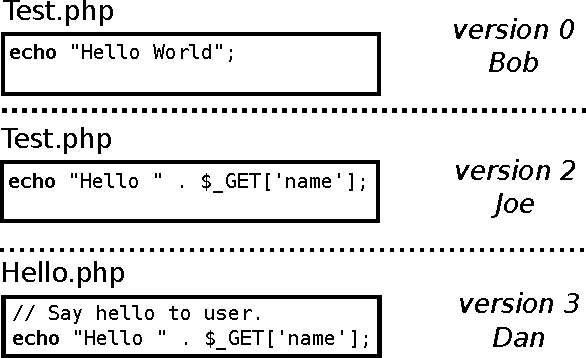
\includegraphics[width=0.8\linewidth,keepaspectratio]{data/figures/example.pdf}
	\caption{Exemple d'un historique de projet. Le projet est composé d'un seul fichier \texttt{Test.php} qui est renommé en \texttt{Hello.php} dans la dernière version.}
	\label{fig:example}
\end{figure}
En ne prenant pas en compte le renommage, la dernière version ne contient qu'une entité. C'est donc cette entité uniquement qui sera considérée. De plus, l'identité exacte de cette entité n'apparaît que lors de la version 3. Le calcul des métriques est donc trivial, NoD$ = 1$.

Par ailleurs, en prenant en compte le fait que ce fichier a été renommé, il y a trois versions à considérer en ce qui concerne l'entité. Le premier nom du fichier était Test.php. Ce fichier a un premier auteur lors de la version 1 puis un deuxième à la version 2. Le fichier est ensuite renommé en Hello.php par un troisième auteur. Le NoD est donc de 3.\\


Intéressons-nous aux outils disponibles pour la gestion de code source. Il existe un certain nombre de gestionnaires de versions tel que SVN, CVS, Mercurial ou Git qui pourraient être compatibles avec notre étude étant donné que nous avons simplement besoin de versions, c'est-à-dire un état du projet à un moment donné de son histoire, à comparer entre elles. Nous avons néanmoins étudié les VCS en détail et découvert que tous ne gèrent pas le renommage de fichiers de la même manière. La ~\tabref{vcs} résume notre étude. Alors que CVS ne gère pas du tout le renommage, SVN ou Mercural propose un mécanisme manuel de détection de renommage de fichiers. Git quant à lui propose un algorithme de détection de renommage automatique et optionnel. Pour les VCS qui utilisent une détection manuelle, cela implique que c'est aux développeurs d'utiliser les commandes appropriées. Cependant certaines études montrent que les développeurs n'utilisent pas ces commandes systématiquement. Le renommage peut être effectué jusqu'à $89\%$ du temps sans utiliser les commandes adaptées ~\cite{lavoie_inferring_2012,steidl_incremental_2014}. De plus l'étude de Kim et al montre que $51$\% des développeurs n'utilisent pas les commandes prévues par le VCS pour le refactoring (incluant le renommage). Ces trois études effectuées sur des projets open-source et industriels, montrent qu'il est dangereux de compter sur le fait que les développeurs utilisent les commandes adéquates pour le refactoring.\\


\subsection{Renommage et VCS}

\begin{table}[h]
\centering
\begin{tabular}{rccc}
\toprule
 & \multicolumn{3}{c}{Renaming handling}\\
\cmidrule{2-4}
& & \multicolumn{2}{c}{Automatic}\\
\cmidrule{3-4}
Tool & Manual & Standard & Optional\\
\midrule
CVS & & &\\
Subversion & $\times$ & &\\
Mercurial & $\times$ & & $\times$\\
Git & & & $\times$\\
\bottomrule
\end{tabular}
\caption{Traitement du renommage des principaux VCS.}
\label{tab:vcs}
\end{table}


\subsection{``Origin Analysis''}

Nous expliquons ici succinctement l'algorithme utilisé par Git pour la détection de renommage de fichiers. Celui-ci est connu sous le nom de ``Origin Analysis'' et est expliqué par Godfrey et al dans les articles ~\cite{tu_integrated_2002,godfrey_tracking_2002,godfrey_using_2005}.

Tout d'abord, il faut considérer deux versions successives d'un projet. Deux ensembles d'entités (fichiers, fonctions..) qui composent leurs versions respectives. Certaines entités ayant été modifiées, certaines supprimées et d'autres ajoutées.
La première analyse est une analyse de Bertillonage qui consiste à choisir un nombre de métriques, puis comparer les entités avec ces métriques. On compare alors les entités supprimées avec les entités ajoutées d'une version à l'autre. Grace à la distance Euclidienne calculée à partir des métriques combinés avec une comparaison des noms des entités, nous obtenons une liste des renommages potentiels.

Les analyses suivantes expliquées par Godfrey sont des améliorations de la première analyse, mais qui ne sont efficaces qu'à un niveau de granularité plus bas, c'est à dire une finesse d'analyse plus précise, en l'occurence au niveau des fonctions. Par exemple, l'analyse de dépendance qui traque les appels de fonctions, en comparant les fonctions appelantes et appelées. Ces analyses sont basées sur des seuils d'acceptabilité défini par l'utilisateur. Plus Godrey améliorera ces analyses, en prenant en compte par la suite les splits er merges de fonctions (algorithme inefficace au niveau des fichiers) plus l'utilisateur sera sollicité. (TODO: détailler ?)\\
